\chapter{Performance of Our Driver}
\label{chap:performance}

\section{First Experiments}
\label{chap:performance.firstexperiments}

\section{Final Experimental Setup}
\label{chap:performance.finalsetup}
\begin{figure}[htb!]
	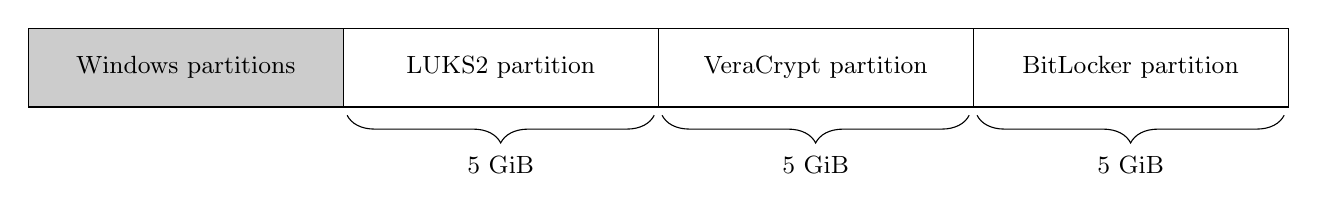
\begin{tikzpicture}
		\draw [fill={gray!40}] (0, 0) rectangle (4, 1);
		\node [anchor=center] at (2, 0.5) {\small\makecell{Windows partitions}};
		\draw [fill=white] (4, 0) rectangle (8, 1);
		\node [anchor=center] at (6, 0.5) {\small\makecell{LUKS2 partition}};
		\draw [fill=white] (8, 0) rectangle (12, 1);
		\node [anchor=center] at (10, 0.5) {\small\makecell{VeraCrypt partition}};
		\draw [fill=white] (12, 0) rectangle (16, 1);
		\node [anchor=center] at (14, 0.5) {\small\makecell{BitLocker partition}};

		\draw [decorate, decoration={brace, amplitude=10pt, mirror}, yshift=-3pt]
		(4.05, 0) -- (7.95, 0) node [black, midway, yshift=-18pt] {\small 5 GiB};
		\draw [decorate, decoration={brace, amplitude=10pt, mirror}, yshift=-3pt]
		(8.05, 0) -- (11.95, 0) node [black, midway, yshift=-18pt] {\small 5 GiB};
		\draw [decorate, decoration={brace, amplitude=10pt, mirror}, yshift=-3pt]
		(12.05, 0) -- (15.95, 0) node [black, midway, yshift=-18pt] {\small 5 GiB};
	\end{tikzpicture}
	\caption[
		Disk layout of the real hardware SSD
	]{
		Disk layout of the real hardware SSD.
	}
	\label{fig:performance.finalsetup.disklayoutssd}
\end{figure}

\section{Results}
\label{chap:performance.results}
For testing purposes, we tried optimizing the performance by restricting support to AES256-XTS. This enabled removing some if-else constructs that dispatched de-/encryption functions based on whether AES128 or AES256 was used. Even though these conditionals were located in a performance critical section, we saw no speed improvements. Our theory for why this was the case is the following: our driver was only ever used for one LUKS2 partition and therefore always took the same path through the if-else (either always AES128 or always AES256). This trained the CPU's branch prediction on this one specific path. Thus, after a short training phase, the CPU always speculatively executed the correct path, resulting in the same performance as without the if-else.

The default compiler optimization settings in Visual Studio were a little bit conservative and also optimized for small code size rather than high speed/performance. After tuning these settings to enable more aggressive optimizations and also focus on speed rather than code size, we found that \todo{this is a little bit complicated...}.